\documentclass[10pt]{beamer}
\usetheme{Madrid}
%\useoutertheme{split}

\newcommand{\bs}{\boldsymbol}


%\setmadridtemplate{navigation symbols}{}

\title[Parallel spreading and interpolation]{A shared memory parallel implementation of the Eulerian-Lagrangian coupling equations for a Stokes Solver}
\author{Sachin Natesh}
\institute{Courant Institute, NYU}
\date{\today}

\begin{document}
\begin{frame}
\titlepage
\end{frame}

\section[]{}

\begin{frame}
\frametitle{Stokes flow and Eulerian-Lagrangian coupling}
\begin{itemize}
	\item Suppose we have $N_p$ particles with \emph{Lagrangian} coordinates $\bs y_k$ immersed in a Stokes fluid in a triply periodic domain $\Omega$. Consider a uniform grid $G$ on $\Omega$ with spacing $h$. The $N^3$ grid nodes $\bs x \in G$ are called \emph{Eulerian} coordinates.
	\item Given forces $\bs f(\bs y_k)$ on the particles, what is their velocity?
	\begin{equation}\label{stokes}
	\eta \nabla^2 \bs{u}(\bs x) - \nabla p(\bs x) = -\bs f(\bs x),\quad \nabla \cdot \bs u(\bs x) = 0.
	\end{equation}
	\item We need a way to \emph{spread} forces on the particles to the Eulerian grid, solve \eqref{stokes}, and \emph{interpolate} the fluid velocity $\bs u(\bs x)$ locally around each particle:
	\begin{equation}\label{spread}
	\textbf{spread } \forall \bs x \in G:\quad \bs f(\bs x) = \sum_{k=1}^{N_p} \bs f(\bs y_k)\Delta(\bs x - \bs y_k)
	\end{equation}
	\begin{equation}\label{interp}
	\textbf{interpolate } \forall k:\quad \bs v(\bs y_k) = \sum_{\bs x \in G}\bs u(\bs x)\Delta(\bs x - \bs y_k)h^3
	\end{equation}
\end{itemize} 
\end{frame}

\begin{frame}
\frametitle{Domain decomposition}
\begin{columns}
\column{0.5\textwidth}
\begin{itemize}
	\item In \eqref{spread}-\eqref{interp}, $\Delta$ is a \emph{finitely supported, symmetric spreading `kernel'} of width $wh$, for $w \in \mathbb{Z}^{+}$, i.e. if $|x^i- y_k^i| > wh/2$ for $i=1,2$ or $3$, then $\Delta(\bs x - \bs y_k)=0.$
	\item This means a Lagrangian coordinate $\bs y_k$ only `talks' to a certain $w \times w \times w$ subarray of the Eulerian grid $G$. 
	\item All particles above and below $\bs y_k$ and within $h/2$ in $x,y$ talk to the \emph{same} $w \times w \times N$ subarray of $G$ $\Rightarrow$ partition the 3D grid into groups of columns!
	\item Loop over the $w^2$ groups of columns and parallelize over the columns in each group.
\end{itemize}
\column{0.5\textwidth}
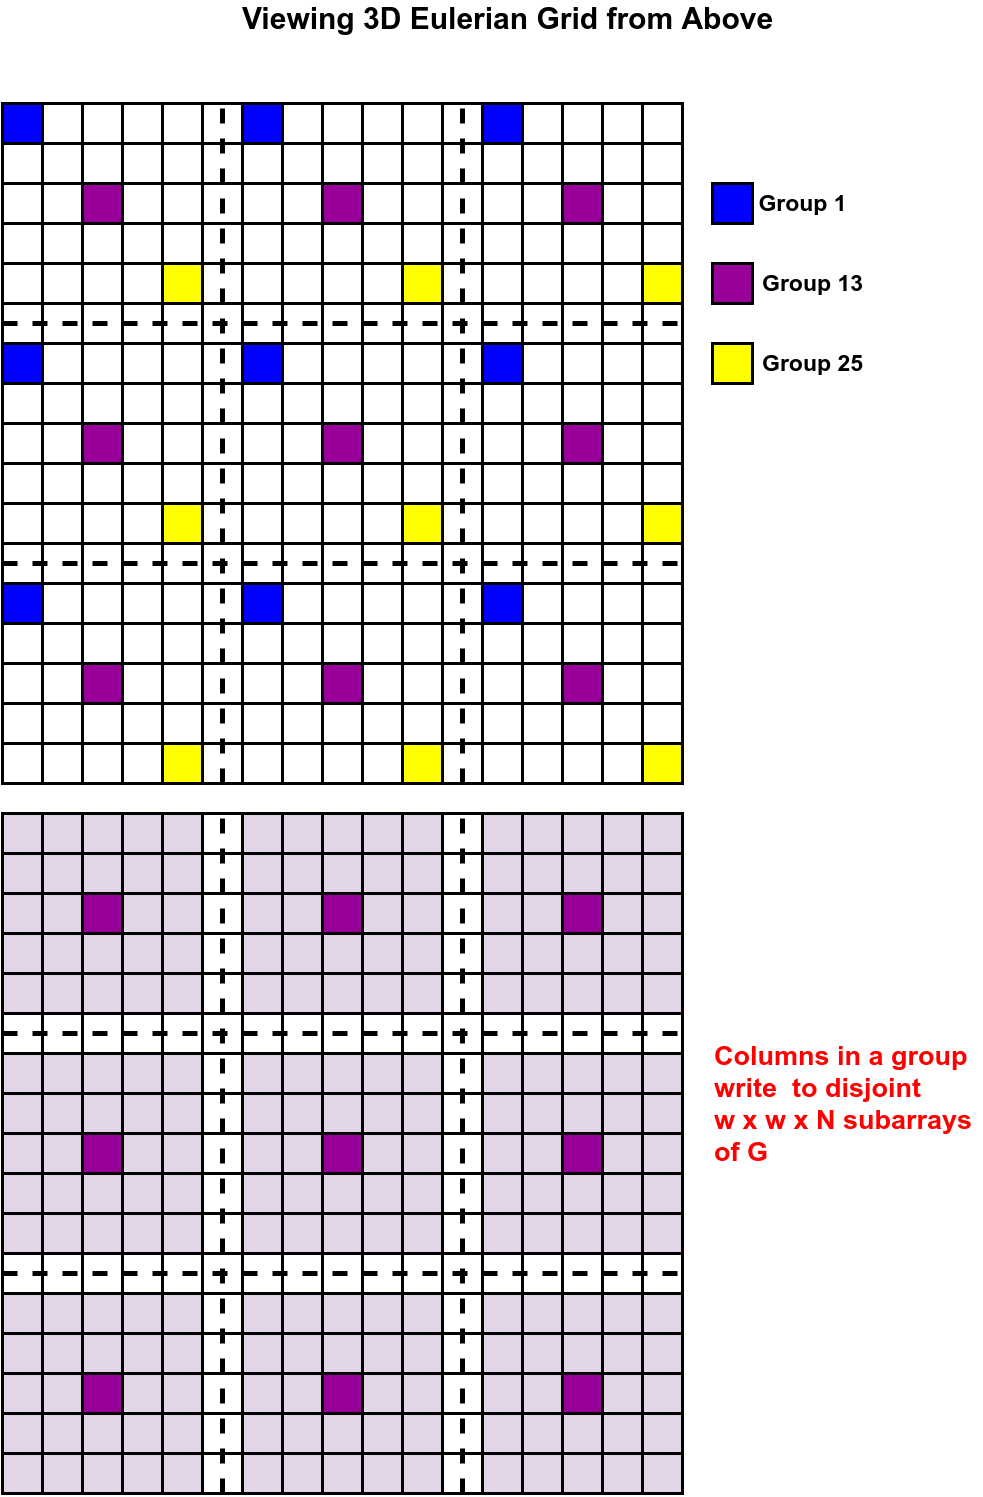
\includegraphics[width=0.8\columnwidth,height=0.8\textheight]{./Figures/domain_decomp_new}
\end{columns}
\end{frame}

\begin{frame}
\frametitle{Algorithm outline}
\begin{enumerate}[1]
	\item Construct an array \texttt{first(i,j)} that gives the \emph{index} $k$ of the first particle in column $i,j$. Along with this, construct an array \texttt{next(k)} that gives the \emph{index} of the \emph{next particle in the column with particle $k$}.
	\item If there is a particle in the column, \texttt{gather} the lagrangian coordinates and forces from the global arrays into cache-aligned local ones.
	\item Compute the global indices of the $w \times w \times N$ subarray of $G$ influenced by the column. Use them to \texttt{gather} the Eulerian forces for one column into cache-aligned memory.
	\item Get the $w \times w \times w$ kernel weights for each particle in the column $\Rightarrow$ vectorize over particles with \texttt{\#pragma omp simd}.
	\item Use the kernel weights and Lagrangian forces to update the Eulerian forces for the column $\Rightarrow$ vectorize over Eulerian points. 
	\item \texttt{scatter} the results back the global Eulerian grid. 
	\item Interpolation is just the weighted adjoint of spreading, so the implementations mirror each other somewhat.
\end{enumerate}
\end{frame}

\begin{frame}
\frametitle{Results}
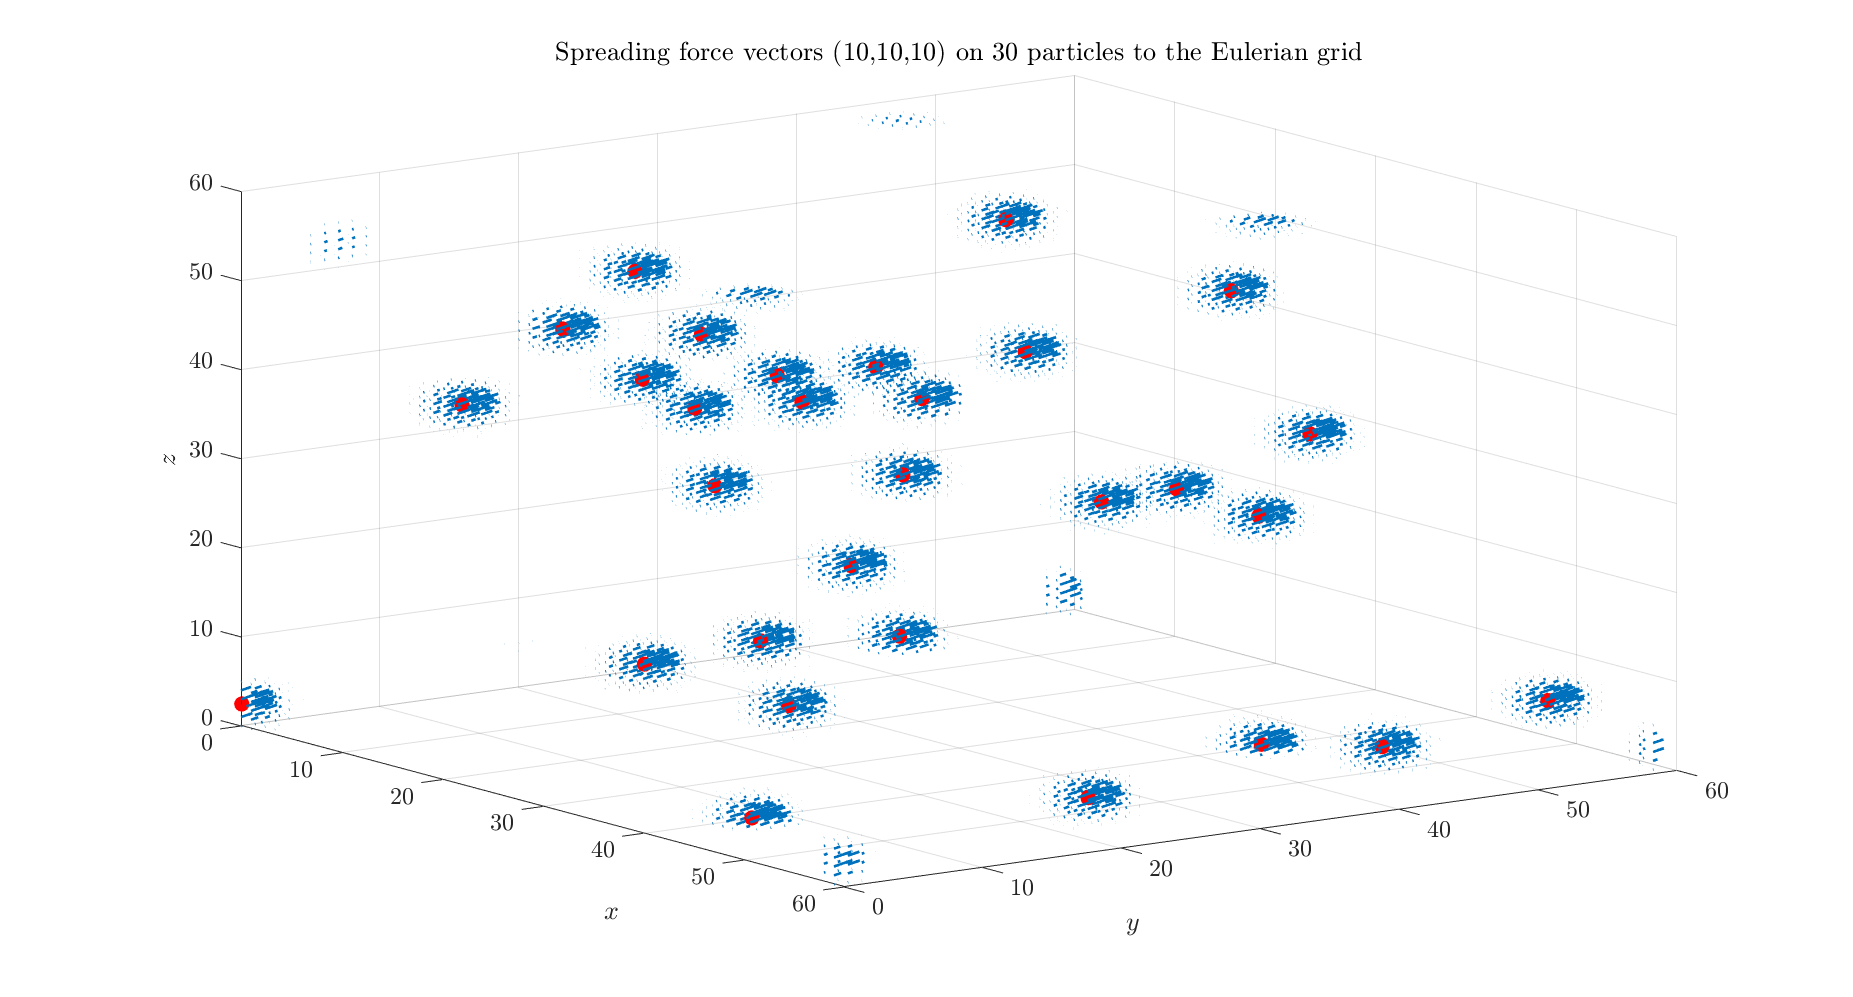
\includegraphics[width=\columnwidth]{./Figures/spread}
\end{frame}
\begin{frame}
\frametitle{Results}
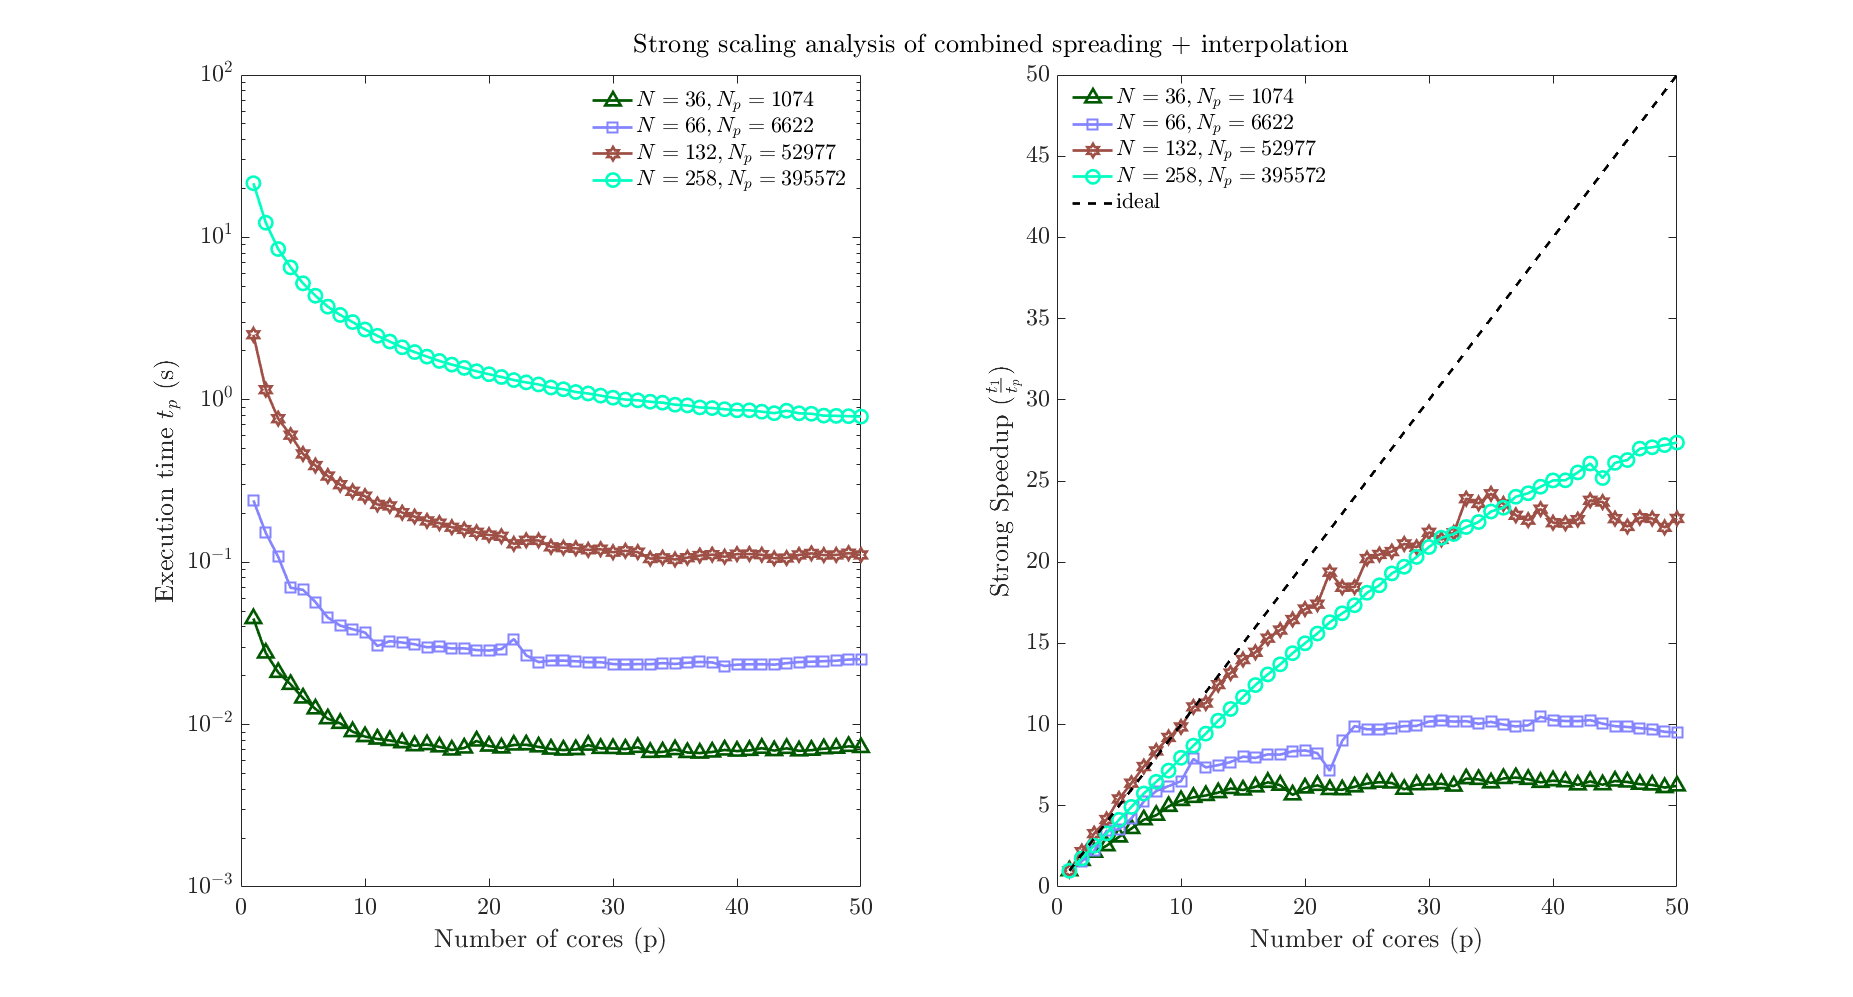
\includegraphics[width=\columnwidth]{./Figures/speedup}
\end{frame}

\begin{frame}
\frametitle{References}
\cite{mcqueen}
\bibliographystyle{amsalpha}
\bibliography{stokes_solver}
\end{frame}



\end{document}